\documentclass[a4paper,11pt]{article}\usepackage[]{graphicx}\usepackage[]{color}
%% maxwidth is the original width if it is less than linewidth
%% otherwise use linewidth (to make sure the graphics do not exceed the margin)
\makeatletter
\def\maxwidth{ %
  \ifdim\Gin@nat@width>\linewidth
    \linewidth
  \else
    \Gin@nat@width
  \fi
}
\makeatother

\definecolor{fgcolor}{rgb}{0.345, 0.345, 0.345}
\newcommand{\hlnum}[1]{\textcolor[rgb]{0.686,0.059,0.569}{#1}}%
\newcommand{\hlstr}[1]{\textcolor[rgb]{0.192,0.494,0.8}{#1}}%
\newcommand{\hlcom}[1]{\textcolor[rgb]{0.678,0.584,0.686}{\textit{#1}}}%
\newcommand{\hlopt}[1]{\textcolor[rgb]{0,0,0}{#1}}%
\newcommand{\hlstd}[1]{\textcolor[rgb]{0.345,0.345,0.345}{#1}}%
\newcommand{\hlkwa}[1]{\textcolor[rgb]{0.161,0.373,0.58}{\textbf{#1}}}%
\newcommand{\hlkwb}[1]{\textcolor[rgb]{0.69,0.353,0.396}{#1}}%
\newcommand{\hlkwc}[1]{\textcolor[rgb]{0.333,0.667,0.333}{#1}}%
\newcommand{\hlkwd}[1]{\textcolor[rgb]{0.737,0.353,0.396}{\textbf{#1}}}%
\let\hlipl\hlkwb

\usepackage{framed}
\makeatletter
\newenvironment{kframe}{%
 \def\at@end@of@kframe{}%
 \ifinner\ifhmode%
  \def\at@end@of@kframe{\end{minipage}}%
  \begin{minipage}{\columnwidth}%
 \fi\fi%
 \def\FrameCommand##1{\hskip\@totalleftmargin \hskip-\fboxsep
 \colorbox{shadecolor}{##1}\hskip-\fboxsep
     % There is no \\@totalrightmargin, so:
     \hskip-\linewidth \hskip-\@totalleftmargin \hskip\columnwidth}%
 \MakeFramed {\advance\hsize-\width
   \@totalleftmargin\z@ \linewidth\hsize
   \@setminipage}}%
 {\par\unskip\endMakeFramed%
 \at@end@of@kframe}
\makeatother

\definecolor{shadecolor}{rgb}{.97, .97, .97}
\definecolor{messagecolor}{rgb}{0, 0, 0}
\definecolor{warningcolor}{rgb}{1, 0, 1}
\definecolor{errorcolor}{rgb}{1, 0, 0}
\newenvironment{knitrout}{}{} % an empty environment to be redefined in TeX

\usepackage{alltt}

\usepackage[left=2.5cm,right=2.5cm,top=3cm,bottom=3cm,pdftex]{geometry}
\usepackage{amssymb, amsmath, url, natbib, float, subcaption, listings,mathtools}
\usepackage[utf8]{inputenc}
\usepackage[T1]{fontenc}
\usepackage[pdftex]{graphicx}

\DeclareGraphicsExtensions{.png, .pdf, .jpg}
\usepackage[pdftex, colorlinks, linkcolor=blue, urlcolor=blue, citecolor=blue, pagecolor=blue, breaklinks=true]{hyperref}
\IfFileExists{upquote.sty}{\usepackage{upquote}}{}
\begin{document}

\pagestyle{empty}
\title{Comparison}
\begin{center}
\Large\textbf{CRAN packages comparison} \\[11pt]
\normalsize
\end{center}

\section{DiffusionRgqd}
Uses the cumulant truncation procedure developed by Varughese (2013), whereby the transition density can be approximated over arbitrarily large transition horizons for a suitably general class of non-linear diffusion models.

Generalized quadratic diffusions (GQD) are the specific class of SDEs with quadratic drift and diffusion terms:

\begin{align*}
d X_t & = \mu(X_t, t)dt + \sigma(X_t, t)dW_t, \: \text{where} \\
\mu(X_t, t) & = G_0(t) + G_1(t) X_t + G_2(t) X_t^2, \: \text{and} \\
\sigma (X_t, t) & = Q_0(t) + Q_1(t) X_t + Q_2(t) X_t^2
\end{align*}

For purposes of inference the drift and diffusion terms - and consequently the transitional density - are assumed to be dependent on a vector of parameters, $\theta$. For example, an Ornstein-Uhlenbeck model with SDE:

\begin{equation}
d X_t = \theta_1 (\theta_2 - X_t) + \sqrt{\theta_3^2} dW_t
\end{equation}

\begin{knitrout}
\definecolor{shadecolor}{rgb}{0.969, 0.969, 0.969}\color{fgcolor}\begin{kframe}
\begin{alltt}
\hlstd{G0}\hlkwb{=}\hlkwa{function}\hlstd{(}\hlkwc{t}\hlstd{)\{theta[}\hlnum{1}\hlstd{]}\hlopt{*}\hlstd{theta[}\hlnum{2}\hlstd{]\}}
\hlstd{G1}\hlkwb{=}\hlkwa{function}\hlstd{(}\hlkwc{t}\hlstd{)\{}\hlopt{-}\hlstd{theta[}\hlnum{1}\hlstd{]\}}
\hlstd{Q0}\hlkwb{=}\hlkwa{function}\hlstd{(}\hlkwc{t}\hlstd{)\{theta[}\hlnum{3}\hlstd{]}\hlopt{*}\hlstd{theta[}\hlnum{3}\hlstd{]\}}
\end{alltt}
\end{kframe}
\end{knitrout}

For a constant drift, diffusion SDE, with given initial condition $X_s$:
\begin{equation}
dX_t = \mu dt + \sigma dW_t
\end{equation}
The distribution at time $t$ of the process $X_t$ is $\mathcal{N}(X_t, X_s + \mu(t-s), \sigma^2(t-s))$

\begin{knitrout}
\definecolor{shadecolor}{rgb}{0.969, 0.969, 0.969}\color{fgcolor}\begin{kframe}
\begin{alltt}
\hlstd{Xs} \hlkwb{<-} \hlnum{0}                 \hlcom{# Initial state}
\hlstd{Xt} \hlkwb{<-} \hlkwd{seq}\hlstd{(}\hlopt{-}\hlnum{3}\hlopt{/}\hlnum{2}\hlstd{,}\hlnum{3}\hlopt{/}\hlnum{2}\hlstd{,}\hlnum{1}\hlopt{/}\hlnum{50}\hlstd{)}\hlcom{# Possible future states}
\hlstd{s}  \hlkwb{<-} \hlnum{0}                 \hlcom{# Starting time}
\hlstd{t}  \hlkwb{<-} \hlnum{1}                 \hlcom{# Final time}
\hlstd{mu}    \hlkwb{<-} \hlnum{0.5}            \hlcom{# Drift parameter}
\hlstd{sigma} \hlkwb{<-} \hlnum{0.25}           \hlcom{# Diffusion coefficient}

\hlkwd{library}\hlstd{(DiffusionRgqd)}
\hlcom{# Remove any existing coefficients:}
\hlkwd{GQD.remove}\hlstd{()}
\end{alltt}
\begin{verbatim}
## [1] "Removed :  G0 G1 Q0"
\end{verbatim}
\begin{alltt}
\hlcom{# Define the model coefficients:}
\hlstd{G0} \hlkwb{<-} \hlkwa{function}\hlstd{(}\hlkwc{t}\hlstd{)\{mu\}}
\hlstd{Q0} \hlkwb{<-} \hlkwa{function}\hlstd{(}\hlkwc{t}\hlstd{)\{sigma}\hlopt{^}\hlnum{2}\hlstd{\}}

\hlcom{# Calculate the transitional density:}
\hlstd{BM} \hlkwb{<-} \hlkwd{GQD.density}\hlstd{(Xs,Xt,s,t)}
\end{alltt}
\begin{verbatim}
##                                                                  
##  ================================================================
##                   Generalized Quadratic Diffusion (GQD)          
##  ================================================================
##  _____________________ Drift Coefficients _______________________
##  G0 : mu                                                         
##  G1                                                              
##  G2                                                              
##  ___________________ Diffusion Coefficients _____________________
##  Q0 : sigma^2                                                    
##  Q1                                                              
##  Q2                                                              
##  __________________ Distribution Approximant ____________________
##  Density approx. : Saddlepoint                                   
##  P               :                                               
##  alpha           :                                               
##  Trunc. Order    : 4                                             
##  Dens.  Order    : 4                                             
## =================================================================
\end{verbatim}
\begin{alltt}
\hlcom{# Plot the transitional density:}
\hlkwd{plot}\hlstd{(}\hlkwd{dnorm}\hlstd{(Xt, Xs}\hlopt{+}\hlstd{mu}\hlopt{*}\hlstd{(t}\hlopt{-}\hlstd{s), sigma}\hlopt{*}\hlkwd{sqrt}\hlstd{(t}\hlopt{-}\hlstd{s))}\hlopt{~}\hlstd{Xt,} \hlkwc{main} \hlstd{=} \hlstr{'Transition density'}\hlstd{,} \hlkwc{type} \hlstd{=} \hlstr{'l'}\hlstd{)}
\hlkwd{lines}\hlstd{(BM}\hlopt{$}\hlstd{density[,}\hlnum{100}\hlstd{]}\hlopt{~}\hlstd{BM}\hlopt{$}\hlstd{Xt,} \hlkwc{col} \hlstd{=} \hlstr{'blue'}\hlstd{,} \hlkwc{lty} \hlstd{=} \hlstr{'dashed'}\hlstd{,} \hlkwc{lwd} \hlstd{=} \hlnum{2}\hlstd{)}
\end{alltt}
\end{kframe}
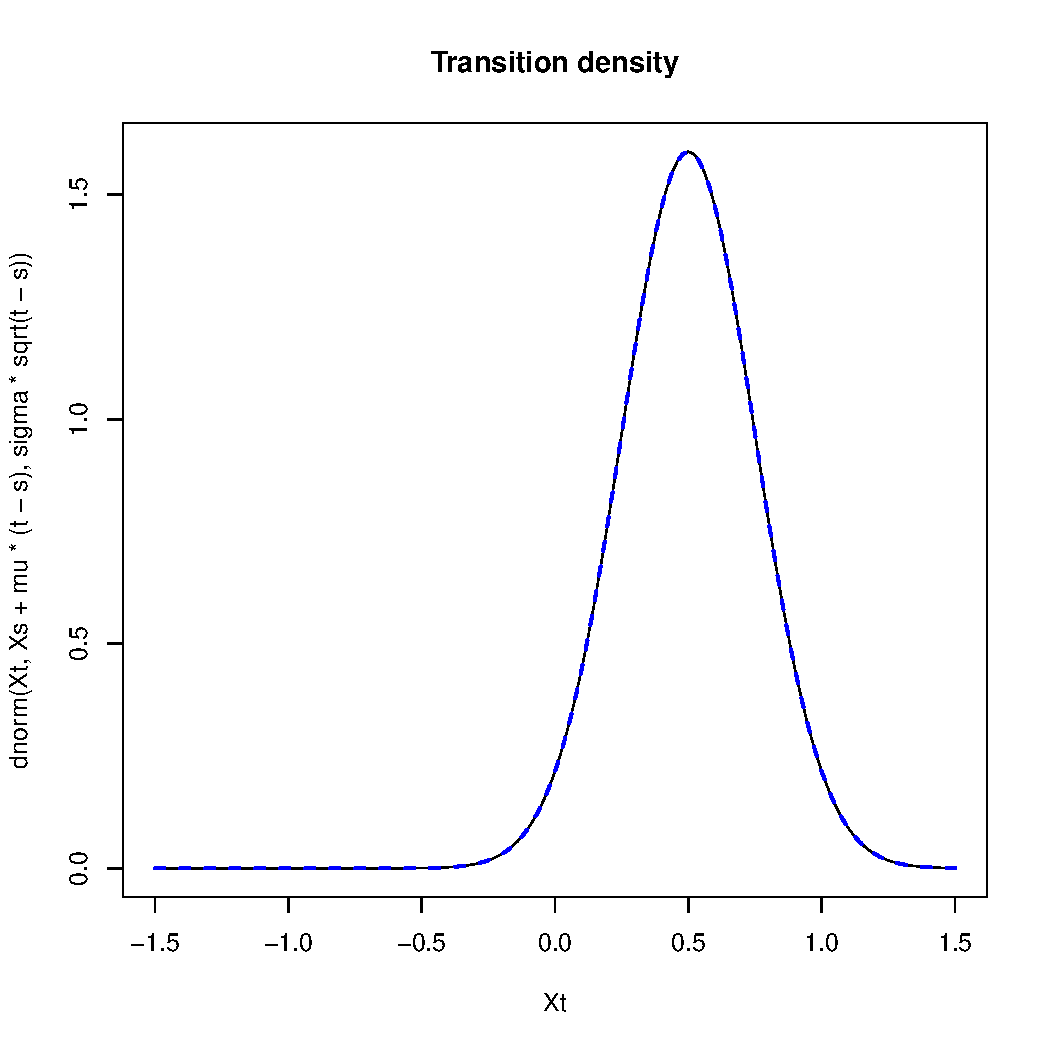
\includegraphics[width=\maxwidth]{figure/Test2-1} 

\end{knitrout}

\end{document}
